% Generated by tools/export_latex.go. Do not edit.
% Per-image phase breakdown of one evaluation pass (pgfplots); Tier 3 is bounded below by the probe window
% Source: empirical_study.json sha256 6102815c4907e01f8b4b5055486eaf0ab1f0140220b9941d0692dd1bbca2a5e1
% Images are chosen at evenly spaced ranks of total duration.
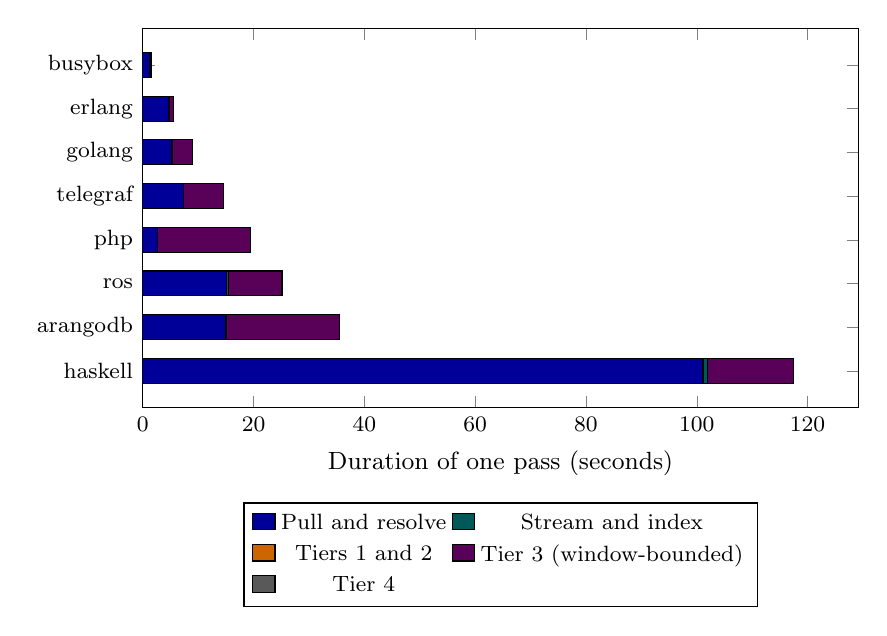
\begin{tikzpicture}
\begin{axis}[
    xbar stacked,
    width=0.88\columnwidth,
    height=6.4cm,
    xlabel={Duration of one pass (seconds)},
    symbolic y coords={busybox,erlang,golang,telegraf,php,ros,arangodb,haskell},
    ytick=data,
    xmin=0,
    enlarge y limits=0.12,
    bar width=9pt,
    y dir=reverse,
    legend style={at={(0.5,-0.25)}, anchor=north, legend columns=2, font=\footnotesize},
    tick label style={font=\footnotesize},
    label style={font=\small},
]
\addplot[fill=blue!60!black] coordinates {
    (1.312,busybox)
    (4.746,erlang)
    (5.158,golang)
    (7.328,telegraf)
    (2.642,php)
    (15.132,ros)
    (14.965,arangodb)
    (101.112,haskell)
};
\addlegendentry{Pull and resolve}
\addplot[fill=teal!70!black] coordinates {
    (0.001,busybox)
    (0.030,erlang)
    (0.133,golang)
    (0.063,telegraf)
    (0.028,php)
    (0.358,ros)
    (0.119,arangodb)
    (0.867,haskell)
};
\addlegendentry{Stream and index}
\addplot[fill=orange!80!black] coordinates {
    (0.000,busybox)
    (0.001,erlang)
    (0.010,golang)
    (0.001,telegraf)
    (0.001,php)
    (0.019,ros)
    (0.002,arangodb)
    (0.016,haskell)
};
\addlegendentry{Tiers 1 and 2}
\addplot[fill=violet!70!black] coordinates {
    (0.250,busybox)
    (0.749,erlang)
    (3.603,golang)
    (7.142,telegraf)
    (16.754,php)
    (9.625,ros)
    (20.362,arangodb)
    (15.432,haskell)
};
\addlegendentry{Tier 3 (window-bounded)}
\addplot[fill=gray!70!black] coordinates {
    (0.000,busybox)
    (0.000,erlang)
    (0.000,golang)
    (0.000,telegraf)
    (0.000,php)
    (0.000,ros)
    (0.000,arangodb)
    (0.000,haskell)
};
\addlegendentry{Tier 4}
\end{axis}
\end{tikzpicture}
